\documentclass[11pt]{article}
\usepackage[scaled=0.92]{helvet}
\usepackage{geometry}
\geometry{letterpaper,tmargin=1in,bmargin=1in,lmargin=1in,rmargin=1in}
\usepackage[parfill]{parskip} % Activate to begin paragraphs with an empty line rather than an indent %\usepackage{graphicx}
\usepackage{amsmath,amssymb, mathrsfs,  mathtools, dsfont}
\usepackage{tabularx}
\usepackage{tikz-cd}
\usepackage[font=footnotesize,labelfont=bf]{caption}
\usepackage{graphicx}
\usepackage{xcolor}
%\usepackage[linkbordercolor ={1 1 1} ]{hyperref}
%\usepackage[sf]{titlesec}
\usepackage{natbib}
%\usepackage{tikz-cd}

\usepackage{../../Tianpei_Report}

%\usepackage{appendix}
%\usepackage{algorithm}
%\usepackage{algorithmic}

%\renewcommand{\algorithmicrequire}{\textbf{Input:}}
%\renewcommand{\algorithmicensure}{\textbf{Output:}}



\begin{document}
\title{Lecture 5: Concentration of Measure and Isoperimetry}
\author{ Tianpei Xie}
\date{Jan. 19th., 2023 }
\maketitle
\tableofcontents
\newpage
\section{The Classic Isoperimetry Inequalities}
\subsection{Brunn-Minkowski Inequality}
\begin{itemize}
\item \begin{definition} (\textbf{\emph{Minkowski Sum of Sets}})\\
Consider sets $A, B \subseteq \bR^n$ and define \underline{\emph{\textbf{the Minkowski sum}}} of $A$ and $B$ as the set of all vectors in $\bR^n$ formed by sums of elements of $A$ and $B$:
\begin{align*}
A + B &:= \set{x+y: x \in A, y \in B}
\end{align*} 
Similarly, for $c \in \bR$, let $c A = \set{cx : x \in A}$. Denote by $\text{Vol}(A)$ the \emph{\textbf{Lebesgue measure}} of a \emph{(measurable) set $A \subset \bR^n$}.
\end{definition}


\item \begin{theorem} (\textbf{Brunn-Minkowski Inequality}) \citep{boucheron2013concentration, vershynin2018high, wainwright2019high}\\
Let $A, B \subset \bR^n$ be \textbf{non-empty compact sets}. Then for all $\lambda \in [0, 1]$,
\begin{align}
\text{Vol}\paren{ \lambda A + (1- \lambda) B }^{\frac{1}{n}} &\ge \lambda\text{Vol}(A)^{\frac{1}{n}} + (1- \lambda)\text{Vol}(B)^{\frac{1}{n}}.   \label{ineqn: brunn_minkowski_inequality}
\end{align}
\end{theorem}
Note:  a convex body in $\bR^n$ is closed and compact set.
\begin{proof} (\textbf{\emph{Part 1, $n = 1$}})\\
Note that if $A \subset \bR$, and $c \ge 0$ then $\text{Vol}(cA) = c\text{Vol}(A)$. Thus it suffice to prove
\begin{align*}
\text{Vol}\paren{  A + B } &\ge \text{Vol}(A) + \text{Vol}(B).
\end{align*} To see this, observe that none of the three volumes involved changes if the sets $A$ and $B$ are \emph{\textbf{translated}} arbitrarily. Since $A, B$ are compact subsets in $\bR$, it is closed and bounded. Let $a = \max\{a': a' \in A\}$ and $b = \min\set{b': b' \in B}$. Let $A' = A +\set{-a}$ and $B' = B + \set{-b}$ so that $A' \subset (-\infty, 0]$ and $B' \subset [0, +\infty)$. Also $\text{Vol}(A') = \text{Vol}(A)$ and $\text{Vol}(B') = \text{Vol}(B)$. 
However, 
\begin{align*}
A' \cup B' &\subset A' + B' \\
\Rightarrow \text{Vol}(A') + \text{Vol}(B') = \text{Vol}(A' \cup B' ) &\le \text{Vol}(A' + B')
\end{align*} This prove the $1$-dimensional case for \emph{the Brunn-Minkowski inequality}. \qed

To prove $n > 1$ case, we need the following inequalities: 
\end{proof}

\item \begin{theorem} (\textbf{The Pr{\'e}kopa-Leindler Inequality}). \citep{boucheron2013concentration, wainwright2019high} \\
Let $\lambda \in (0, 1)$, and let $f, g, h : \bR^n \to [0, \infty)$ be \textbf{non-negative measurable functions} such that for all $x, y \in \bR^n$,
\begin{align*}
h\paren{\lambda x + (1- \lambda) y} &\ge f(x)^{\lambda}g(y)^{1-\lambda}.
\end{align*} Then
\begin{align}
\int_{\bR^n} h(x) dx &\ge \paren{\int_{\bR^n} f(x) dx }^{\lambda}\paren{\int_{\bR^n} g(x) dx}^{1-\lambda}.   \label{ineqn: prekopa_leindler_inequality}
\end{align}
\end{theorem}
\begin{proof}
The proof goes by induction with respect to the dimension $n$.
\begin{enumerate}
\item (\textbf{\emph{$n=1$ case}}). Consider measurable non-negative functions $f, g, h$ satisfying the condition of the theorem. By \emph{the monotone convergence theorem}, it suffices to prove the statement for \emph{\textbf{bounded functions}} $f$ and $g$.  Without loss of generality, assume that  $\sup_{x\in \bR^n} f(x) = \sup_{x\in \bR^n} g(x) = 1$.  Then
\begin{align*}
\int_{\bR} f(x) dx &= \int_{0}^{1}\text{Vol}\set{x: f(x) \ge t} dt \\
\int_{\bR} g(x) dx &= \int_{0}^{1}\text{Vol}\set{x: g(x) \ge t} dt.
\end{align*} For any fixed $t \in [0, 1]$, if $f(x) \ge t$ and $g(y) \ge t$, then by the hypothesis of the theorem, $h\paren{\lambda x + (1- \lambda) y} \ge t$. This implication may be re-written as
\begin{align*}
\lambda\set{x: f(x) \ge t} + (1- \lambda) \set{x: g(x) \ge t} &\subset \set{x: h(x) \ge t}.
\end{align*} Thus
\begin{align*}
\int_{\bR} h(x) dx &= \int_{0}^{\infty}\text{Vol}\set{x: h(x) \ge t} dt \\
&\ge  \int_{0}^{1}\text{Vol}\set{x: h(x) \ge t} dt \\
&\ge \int_{0}^{1} \text{Vol}\paren{\lambda\set{x: f(x) \ge t}} + \text{Vol}\paren{(1- \lambda) \set{x: g(x) \ge t}} dt \\
& (\text{ by $1$-dimensional \emph{Brunn-Minkowski inequality}}) \\
&\ge \lambda \int_{0}^{1}\text{Vol}\paren{\set{x: f(x) \ge t}}dt + (1- \lambda)\int_{0}^{1}\text{Vol}\paren{ \set{x: g(x) \ge t}}dt \\
& =\lambda   \int_{\bR} f(x) dx  + (1- \lambda) \int_{\bR} g(x) dx \\
&\ge \paren{\int_{\bR} f(x) dx }^{\lambda}\paren{\int_{\bR} g(x) dx}^{1-\lambda} \; \text{(by the \emph{arithmetic-geometric mean inequality})}
\end{align*}

\item For the induction step, assume that the theorem holds for all dimensions $1 \xdotx{,} n - 1$ and let $f, g, h : \bR^n \to [0, \infty)$,  $\lambda \in (0, 1)$ be such that they satisfy the assumption of the theorem.  Now let $x, y \in \bR^{n-1}$ and $a, b \in \bR$. Then
\begin{align*}
h\paren{\lambda \paren{x, a} + (1-\lambda)\paren{y, b}} \ge f\paren{(x, a)}^{\lambda} g((y, b))^{1- \lambda}, 
\end{align*} so by the inductive hypothesis
\begin{align*}
\int_{\bR^{n-1}} h\paren{(x, \lambda a + (1-\lambda) b)} dx &\ge \paren{\int_{\bR^{n-1}} f\paren{(x, a)} dx}^{\lambda}\paren{\int_{\bR^{n-1}} g((x, b)) dx }^{1- \lambda} 
\end{align*} In other words, introducing
\begin{align*}
F(a) := \int_{\bR^{n-1}} f\paren{(x, a)} dx, \quad G(b) := \int_{\bR^{n-1}} g((x, b)) dx\\
H((\lambda a + (1-\lambda) b)) := \int_{\bR^{n-1}} h\paren{(x, \lambda a + (1-\lambda) b)} dx.
\end{align*} We have
\begin{align*}
H((\lambda a + (1-\lambda) b))  &\ge \paren{F(a)}^{\lambda}\paren{G(b)}^{1- \lambda},
\end{align*} so by \emph{Fubini's theorem} and the one-dimensional inequality, we have
\begin{align*}
\int_{\bR^n}h(x) dx =  \int_{\bR} H(a)   da &\ge \paren{\int_{\bR} F(a) da}^{\lambda}\paren{\int_{\bR} G(a) da}^{1 - \lambda} \\
&= \paren{\int_{\bR^n} f(x) dx}^{\lambda}\paren{\int_{\bR^n} g(x) dx}^{1 - \lambda}.  \qed
\end{align*}
\end{enumerate} 
\end{proof}

\item \begin{corollary} (\textbf{Weaker Brunn-Minkowski Inequality}) \citep{boucheron2013concentration, wainwright2019high}\\
Let $A, B \subset \bR^n$ be \textbf{non-empty compact sets}. Then for all $\lambda \in [0, 1]$,
\begin{align}
\text{Vol}\paren{ \lambda A + (1- \lambda) B } &\ge \text{Vol}(A)^{\lambda}\text{Vol}(B)^{1- \lambda}.   \label{ineqn: brunn_minkowski_inequality_weaker}
\end{align}
\end{corollary}
\begin{proof}
We apply \emph{the Pr{\'e}kopa-Leindler inequality} with $f(x) = \ind{x \in A}$, $g(x) = \ind{x \in B}$ and $h(x) = \ind{x \in \lambda A + (1- \lambda) B}$. We see that 
\begin{align*}
h(\lambda x + (1- \lambda) y) &= \ind{\lambda x + (1- \lambda) y \in \lambda A + (1- \lambda) B} \ge \ind{x \in A, y \in B}  = f(x)^{\lambda}g(y)^{1 - \lambda}.
\end{align*} Thus the hypothesis of \emph{the Pr{\'e}kopa-Leindler inequality} holds. \qed
\end{proof}

\item \begin{proof}  (\textbf{\emph{$n> 1$ case for Brunn-Minkowski Inequality}}).  First observe that it suffices to prove that for all \emph{nonempty compact sets} $A$ and $B$,
\begin{align*}
\text{Vol}\paren{ A + B }^{\frac{1}{n}} &\ge \text{Vol}(A)^{\frac{1}{n}} + \text{Vol}(B)^{\frac{1}{n}}
\end{align*} since $\text{Vol}\paren{c A}^{1/n} = c \text{Vol}\paren{A}^{1/n}$ for any $c \in \bR$ and $A \subset \bR^n$. Also notice that we may assume that $ \text{Vol}(A),  \text{Vol}(B) > 0$ because otherwise the inequality holds trivially. Defining $A' = \text{Vol}(A)^{-\frac{1}{n}} A$ and $B' =  \text{Vol}(B)^{-\frac{1}{n}}B$, we have $ \text{Vol}(A') = \text{Vol}(B') = 1$. By \emph{weaker Brunn-Minkowski inequality}, for $\lambda \in (0, 1)$,
\begin{align*}
\text{Vol}\paren{ \lambda A' + (1- \lambda) B' } &\ge 1.
\end{align*} Finally, we apply this \emph{inequality} with the choice
\begin{align*}
\lambda &= \frac{\text{Vol}(A)^{\frac{1}{n}}}{\text{Vol}(A)^{\frac{1}{n}} + \text{Vol}(B)^{\frac{1}{n}}}
\end{align*} obtaining
\begin{align*}
\text{Vol}\paren{ \frac{\text{Vol}(A)^{\frac{1}{n}}A'}{\text{Vol}(A)^{\frac{1}{n}} + \text{Vol}(B)^{\frac{1}{n}}}  + \frac{\text{Vol}(B)^{\frac{1}{n}}B'}{\text{Vol}(A)^{\frac{1}{n}} + \text{Vol}(B)^{\frac{1}{n}}}  }  &\ge 1\\
\Rightarrow \text{Vol}\paren{ \frac{A}{\text{Vol}(A)^{\frac{1}{n}} + \text{Vol}(B)^{\frac{1}{n}}}  + \frac{B}{\text{Vol}(A)^{\frac{1}{n}} + \text{Vol}(B)^{\frac{1}{n}}}  }  &\ge 1 \\
\Rightarrow \text{Vol}\paren{ \frac{A + B}{\text{Vol}(A)^{\frac{1}{n}} + \text{Vol}(B)^{\frac{1}{n}}}    }  &\ge 1 \\
\Rightarrow \frac{\text{Vol}(A + B)}{\paren{\text{Vol}(A)^{\frac{1}{n}} + \text{Vol}(B)^{\frac{1}{n}}}^n} &\ge 1 
\end{align*} which proves the theorem. \qed
\end{proof}
\end{itemize}

\subsection{The Blowup of Sets and Classical Isoperimetry Theorem}
\begin{itemize}
\item \begin{definition} (\textbf{\emph{Blowup of Sets}}) \\
For any $t > 0$, and any (measurable) sets $A \subset \bR^n$,  \emph{\underline{\textbf{the $t$-blowup}} of $A$} is defined by
\begin{align*}
A_t &:= \set{x \in \bR^n: d(x, A) < t} = A + t\,B
\end{align*} where $B = \set{x \in \bR^n: d(0, x) < 1}$ is an \emph{open unit ball} and $d(x, A) = \inf_{y \in A}d(x, y)$.
\end{definition}

\item \begin{definition}(\textbf{\emph{Surface Area of Sets}}) \\
let $A \subset \bR^n$ be a measurable set and denote by $\text{Vol}(A)$ its \emph{Lebesgue measure}. \emph{The  \underline{\textbf{surface area}} of $A$} is
defined by
\begin{align*}
\text{Vol}(\partial A) &= \lim\limits_{t \to 0}\frac{\text{Vol}(A_t) - \text{Vol}(A)}{t}.
\end{align*} provided that the limit exists. Here $A_t$ denotes \emph{the $t$-blowup} of $A$.
\end{definition}

\item \begin{remark}(\textbf{\emph{Isoperimetry Theorem}})\\
The classical isoperimetric theorem in $\bR^n$ states that, among all sets with \emph{\textbf{a given volume}}, \underline{\emph{\textbf{the Euclidean unit ball minimizes the surface area}}}.  This theoerm can be formally stated as below:
\end{remark}

\begin{figure}
\begin{minipage}[t]{1\linewidth}
  \centering
  \centerline{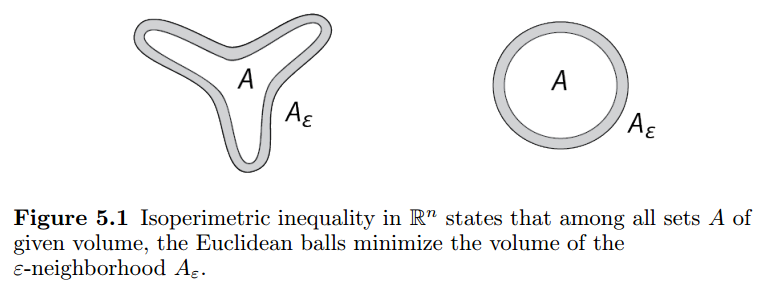
\includegraphics[scale = 0.4]{isoperimetry_rn.png}}
\end{minipage}
\caption{\footnotesize{\textbf{Isoperimetry in $\bR^{n}$  \citep{vershynin2018high}}}}
\label{fig: isoperimetry_rn}
\end{figure}


\item \begin{theorem} (\textbf{Isoperimetry Theorem}) \citep{boucheron2013concentration, vershynin2018high, wainwright2019high}\\
Let $A \subset \bR^n$ be such that $\text{Vol}(A) = \text{Vol}(B)$ where $B := \set{x \in \bR^n: d(0, x) < 1}$ is an unit ball. Then for any $t > 0$, 
\begin{align}
\text{Vol}(A_t) &\ge  \text{Vol}(B_t) \label{ineqn: isoperimetry_inequality_blowup}
\end{align} Moreover, if $\text{Vol}(\partial A) $ exists, then
\begin{align}
\text{Vol}(\partial A)  &\ge \text{Vol}(\partial B).  \label{ineqn: isoperimetry_inequality_surface}
\end{align}
\end{theorem}
\begin{proof}
By \emph{the Brunn-Minkowski inequality}, 
\begin{align*}
\text{Vol}(A_t)^{1/n}  = \text{Vol}(A + tB)^{1/n} &\ge \text{Vol}(A)^{1/n} +  t\text{Vol}(B)^{1/n} \\
&= (1+t) \text{Vol}(B)^{1/n} \\
&= \text{Vol}(B_t)^{1/n},
\end{align*} establishing the first statement. The second follows simply because
\begin{align*}
\text{Vol}(A_t) - \text{Vol}(A) &\ge \text{Vol}(B)((1+t)^n -1) \ge nt\text{Vol}(B)
\end{align*} where $(1+t)^n \ge 1 + nt$ for $t \ge 0$. Thus $\text{Vol}(\partial A)  \ge n\text{Vol}(B)$. The isoperimetric theorem now follows from the fact that
$\text{Vol}(\partial B) = n\text{Vol}(B)$. \qed
\end{proof}
\end{itemize}

\section{Concentration via Isoperimetry}
\subsection{Levy's Inequalities}
\begin{itemize}
\item \begin{remark}
We can generalize the classical isoperimety problem to a probability space $(\cX, \cB[\cX], \bP)$ where $\cX$ is a \emph{metric space} with metric $d$, $\cB[\cX]$ is the Borel $\sigma$-algrebra and $\bP$ is a probability measure on $\cB[\cX]$. Let  $B := \set{x \in \bR^n: d(0, x) < 1}$. The classical isoperimetry problem aims at finding the set $A^{*} \subset \cX$ that \emph{\textbf{minimizes the surface area}}
\begin{align*}
\bP(\partial A) = \lim\limits_{t \to 0}\frac{\bP(A_t) - \bP(A)}{t}
\end{align*} This is equivalent to find subset $A$ in $\cX$ with \emph{\textbf{minimal $t$-blowup}} for given $p$, and for all $t >0$
\begin{align*}
A^{*} := \inf_{A \subset \cX: \bP(A) \ge p}\bP(A_t), \quad \forall t > 0
\end{align*} where 
\begin{align*}
A_t = A + tB = \set{x \in \cX:  \exists y \in A \text{ s.t. } d(x, y) < t} = \set{x \in \cX:  \inf_{y \in A}d(x, y) := d(x, A) < t}.
\end{align*} We write the definition formally.
\end{remark}


\item \begin{definition} (\emph{\textbf{Isoperimetry Problem}}) \citep{boucheron2013concentration}\\
Given a \emph{\textbf{metric space}} $\cX$ with corresponding \emph{distance} $d$, consider \emph{\textbf{the measure space}} formed by $\cX$ , \emph{the $\sigma$-algebra} of all \emph{\textbf{Borel sets} of $\cX$}, and a probability measure $\bP$. Let $X$ be a \emph{random variable} taking values in $\cX$, distributed according to $\bP$. 

\underline{\emph{\textbf{The isoperimetric problem}}} in this case is the following: given $p \in (0, 1)$ and $t > 0$, \emph{\textbf{determine the sets}} $A$ with $\bP\brac{X \in A} \ge p$ for which \emph{the measure}
\begin{align*}
\bP\brac{d(X, A) \ge t}
\end{align*}  is \emph{\textbf{maximal}}. 
\end{definition}

\item \begin{remark} (\emph{\textbf{Isoperimetric Inequalities}})\\
Even though the exact solution is only known in a few special cases, useful \emph{bounds} for $\bP\brac{d(X, A) \ge t}$ can be derived under remarkably general circumstances. \emph{Such bounds are usually referred to as} \underline{\emph{\textbf{isoperimetric inequalities}}}.
\end{remark}

\item \begin{definition} (\textbf{\emph{Concentration Function}}) \citep{boucheron2013concentration, wainwright2019high}\\
\underline{\emph{\textbf{The concentration function}}} $\alpha: [0, \infty) \to \bR_{+}$  associated with \emph{\textbf{metric measure space}} $((\cX, d), \bP)$ is given by
\begin{align*}
\alpha_{\bP, (\cX, d)}(t) &:= \sup_{ A \subset \cX:\, \bP\paren{A} \ge \frac{1}{2}}\bP\brac{d(X, A) \ge t } = \sup_{A \subset \cX: \,\bP\paren{A} \ge \frac{1}{2}}\bP\paren{A_{t}^{c} }
\end{align*} where $A_t:= A + tB = \set{x \in \cX: d(x, A) < t}$ is \emph{the $t$-blowup} of $A \subset \cX$. We simply denote it as $\alpha(t)$.
\end{definition}
Thus the optimal $A^{*}$ for isoperimetry problem is the one that attains the $\alpha(t) = \bP\paren{A_{t}^{c} }$.

\item \begin{theorem} (\textbf{Levy's Inequalities})\citep{boucheron2013concentration, wainwright2019high}\\
For any Lipschitz function $f: \cX \to \bR$, 
\begin{align}
\bP\set{f(X) \ge  \text{Med}(f(X)) + t } &\le \alpha_{\bP}(t) \label{ineqn: levy_inequality}\\
\bP\set{f(X)  \le  \text{Med}(f(X))  -  t } &\le \alpha_{\bP}(t).  \nonumber
\end{align} where $\text{Med}(f(X))$ is \underline{\textbf{the median} of $f(X)$}, i.e.
\begin{align*}
\bP\set{f(X) \le \text{Med}(f(X)} \ge  \frac{1}{2}, \;\text{ and }\; \bP\set{f(X) \ge \text{Med}(f(X)} \ge  \frac{1}{2}.
\end{align*}
\end{theorem}
\begin{proof} 
Consider the set $A = \set{x : f(x) \le \text{Med}(f(X))}$. By the definition of a \emph{median},  $\bP\paren{A} \ge \frac{1}{2}$. On the other hand, by \emph{the Lipschitz property} of $f$, for any $x, y \in \cX$,
\begin{align*}
\abs{f(x) - f(y)} \le d(x, y). 
\end{align*} So for all $y \in A$,  $f(y) \le \text{Med}(f(X))$
\begin{align*}
f(x) -  \text{Med}(f(X))  &\le f(x) - f(y) \le d(x, y) \\
\Rightarrow  f(x) -  \text{Med}(f(X))  &\le \inf_{y \in A}d(x, y) := d(x, A).
\end{align*} Equivalently, 
\begin{align*}
A_t := \set{x \in \cX: d(x, A) < t} &\subseteq \set{x \in \cX:  f(x) < \text{Med}(f(X)) + t } \\
\bP(A_t^{c}) &\ge \bP\set{ f(X) \ge \text{Med}(f(X)) + t } 
\end{align*} The first inequality now follows from the definition of the concentration function.  The second inequality follows from the first by considering $–f$.  \qed
\end{proof}

\item \begin{remark} For $L$-Lipschitz function $f$, the inequality becomes
\begin{align*}
\bP\set{f(X) - \text{Med}(f(X)) \ge t } \le  \alpha\paren{\frac{t}{L}}, \quad \bP\set{f(X) - \text{Med}(f(X)) \le -t } &\le \alpha\paren{\frac{t}{L}}.
\end{align*}
\end{remark}

\item \begin{theorem}  (\textbf{Converse of Levy's Inequalities})\citep{boucheron2013concentration, wainwright2019high}\\
If $\beta : \bR_{+} \to [0, 1]$ is a function such that for \textbf{every Lipschitz function} $f : \cX \to \bR$
\begin{align}
\bP\set{f(X) - \text{Med}(f(X)) \ge t } &\le \beta(t). \label{ineqn: converse_levy_inequality}
\end{align} then $\beta(t) \ge \alpha_{\bP}(t)$.
\end{theorem}
\begin{proof}
Note that for any $A \subset \cX$ , the function $f_A$ defined by $f_A(x)= d(x, A)$ is \emph{Lipschitz} since
\begin{align*}
\abs{f_A(x) - f_A(y)} = \abs{d(x, A) - d(y, A)} &\le d(x, y).
\end{align*} Also, if  $P\paren{A} \ge 1/2$, then $0$ is a median of $f_A(X)$, since
\begin{align*}
\bP\set{f_A(x) \le 0} = \bP\set{d(X, A) \le 0} = \bP(A) \ge \frac{1}{2}.
\end{align*}  Therefore
\begin{align*}
\alpha(t) := \sup_{A \subset \cX: \bP(A) \ge 1/2}\bP\set{f_A(x) - \text{Med}(f_A(X)) \ge t} \le \beta(t). \qed
\end{align*}
\end{proof}

\item \begin{proposition} (\textbf{Levy's Inequalities for Mean})\citep{boucheron2013concentration, wainwright2019high}\\
If $\beta: \bR_{+} \to [0,1]$ is a  function such that for \textbf{every Lipschitz function} $f : \cX \to \bR$
\begin{align}
\bP\set{f(X) - \E{}{f(X)} \ge t } &\le \beta(t). \label{ineqn: converse_levy_inequality_mean}
\end{align} then $\beta(t) \ge \alpha_{\bP}(t/2)$.
\end{proposition}

\item \begin{remark} (\emph{\textbf{Isoperimetric Inequalities $\Leftrightarrow$ Concentration of Lipschitz Functions}})\\
The first result points out that \emph{isoperimetric inequalities} (more precisely, \emph{\textbf{upper bounds} for \textbf{the concentration function}}) imply
\emph{concentration of Lipschitz functions}. 

\emph{\textbf{The converse}} shows that \emph{concentration of Lipschitz functions} implies an \emph{isoperimetric inequality}. In other word, \emph{among all upper bounds} of $\bP(A_t^c)$ for fixed $A_t$, 
\end{remark}

\item \begin{corollary} (\textbf{Concentration of  Measure on Hamming Metric Space}) \citep{boucheron2013concentration}\\
Consider \emph{independent random variables} $Z_1 \xdotx{,} Z_n$ taking their values in a \emph{(measurable) set} $\cX$ and denote the vector of these variables by $Z = (Z_1 \xdotx{,} Z_n)$ taking its value in $\cX^n$.  For an arbitrary (measurable) set $A \subset \cX^n$, we write $\bP\paren{A} = \bP\paren{Z \in A}$.  The \textbf{Hamming distance} $d_{H}(x, y)$ between the vectors $x, y \in \cX^n$ is defined as \textbf{the number of coordinates} in which $x$ and $y$ \textbf{differ}. Then for any $t >0$, 
\begin{align}
\bP\set{d_{H}(x, A) \ge \sqrt{\frac{n}{2}\log \frac{1}{\bP(A)}} + t} \le \exp\paren{-\frac{2t^2}{n}}  \label{ineqn: isoperimetry_inequality_hamming_distance}
\end{align}
\end{corollary}
\begin{proof}
As we shown in previous proof, $f_A(x) = d_{H}(x, A)$ is a Lipschitz function with respect to Hamming distance $d_H$. It follows from the definition that 
\begin{align*}
\sup_{x \in \cX^n, y_i \in \cX}\abs{f_{A}(x) - f_{A}(\widetilde{x}^{(i)})} \le d_{H}(x, \widetilde{x}^{(i)}) = 1
\end{align*} where $\widetilde{x}^{(i)} = (x_1 \xdotx{,} x_{i-1}, y_i, x_{i+1} \xdotx{,} x_{n})$, so $f_A$ has the bounded difference property. By bounded difference inequality, 
\begin{align*}
\bP\set{ \E{}{f_{A}(Z)} - f_{A}(Z)  \ge t }  &\le \exp\paren{-\frac{2t^2}{n}}.
\end{align*} Taking $t = \E{}{f_{A}(Z)} = \E{}{d_{H}(Z, A)}$, the left-hand side becomes $\bP\set{f_{A}(Z) \le 0} = \bP\set{d_{H}(Z, A)  \le 0}  = \bP\paren{A}$. Then the inequality becomes
\begin{align*}
\bP\paren{A} &\le \exp\paren{- \frac{2}{n} \paren{\E{}{d_{H}(Z, A)}}^2} \\
\Rightarrow \E{}{d_{H}(Z, A)} &\le \sqrt{\frac{n}{2}\log \frac{1}{\bP(A)}}.
\end{align*} Then, by using the bounded difference inequality again, we obtain
\begin{align*}
\bP\set{d_H(Z, A) \ge  \sqrt{\frac{n}{2}\log \frac{1}{\bP(A)}} + t } \le \bP\set{d_H(Z, A) \ge  \E{}{d_{H}(Z, A)} + t } \le \exp\paren{-\frac{2t^2}{n}}. \qed
\end{align*}
\end{proof}


\item \begin{remark} (\textbf{\emph{Concentration of Measure}})\\
To interpret the result in \eqref{ineqn: isoperimetry_inequality_hamming_distance}, we see that on the left-hand side we have the measure of the set of points whose Hamming distance is at least $t + \sqrt{\frac{n}{2}\log \frac{1}{\bP(A)}}$ away from $A$. This inequality means that for $A$ with \emph{\textbf{small measure}} $\bP(A)$, the measure of points whose \emph{\textbf{Hamming distance}} from $A$ is \emph{more than} $O\paren{\sqrt{n}}$ is \emph{\textbf{extremely small}}.

In other words, \emph{\textbf{product measure} on Hamming metric space are \textbf{concentrated} on \textbf{extremely small sets}}. This phenonemon is called ``\underline{\textbf{\emph{concentration of measure}}}". 
\end{remark}

\item \begin{example} (\textbf{\emph{Bounded Difference Property $\Leftrightarrow$ Lipschitz Condition w.r.t. Hamming Distance}}) \\
Note that any  function with \emph{\textbf{bounded difference property}} is \emph{\textbf{Lipschitz function}} with respect to \emph{\textbf{Hamming distance}}. 
\begin{align*}
&\sup_{x \in \cX^n, y_i \in \cX}\abs{f(x_1 \xdotx{,} x_n) - f(x_1 \xdotx{,} x_{i-1}, y_i, x_{i+1} \xdotx{,} x_{n})} &\\
&\le c_i = c_i\,d_{H}((x_1 \xdotx{,} x_n), (x_1 \xdotx{,} x_{i-1}, y_i, x_{i+1} \xdotx{,} x_{n})), \quad 1\le i \le n\\
\Rightarrow \abs{f(x) - f(y)} &=  \abs{\sum_{i=1}^{n}(f(x_{(i-1)}) - f(x_{(i)}) )}\\
&\quad \le  \sum_{i=1}^{n}\abs{f(x_{(i-1)}) - f(x_{(i)}) }\\
&\quad \le \sum_{i=1}^{n}c_i \ind{x_{(i-1)}[i] \neq x_{(i)}[i]} \\
&\quad = d_{H,c}(x, y)
\end{align*}   where $x_{(i)}$ is replicate of $x_{(i-1)}$ except for $i$-th component, which is replaced by $y_i$. Note that $x_{(0)} = x$ and $x_{(n)} = y$. 
Therefore, \emph{the bounded difference inequality} can be seen as \emph{an isoperimetry inequality} for \emph{Lipschitz function with respect to Hamming distance}.
\begin{align*}
 \bP\set{f(Z) - \E{}{f(Z)} \ge t } &\le \exp\paren{-\frac{2t^2}{n}}
\end{align*}
\end{example}


\end{itemize}
\subsection{Isoperimetric Inequalities on the Unit Sphere}
\begin{itemize}
%\item \begin{remark} (\emph{\textbf{Volume Ratio of Unit Balls and its Interior}})  \citep{vershynin2018high}\\
%Let $B(0, 1):= \set{x \in \bR^n: \norm{x}{} \le 1}$ be the unit ball in $\bR^n$. The volume ratio between $B(0,1)$ and its $\epsilon$-interior $B(0, 1-\epsilon)$ is
%\begin{align*}
%\frac{\text{Vol}(B(0, 1-\epsilon))}{\text{Vol}(B(0,1))} &= (1 - \epsilon)^n \le \exp\paren{-n \epsilon}
%\end{align*} The inequality is due to $1 - x\le e^{-x}$.  
%
%As $n \to \infty$, the above ratio goes to $0$. In other words, most of volume in $B(0,1)$ is \emph{\textbf{concentrated}} in the \emph{\textbf{boundary}} $\partial B = \bS^{n-1} := \set{x \in \bR^n: \norm{x}{} = 1}$. This phenomenon is called ``\emph{\textbf{the curse of dimensionality}}".
%\end{remark}
\begin{figure}
\begin{minipage}[t]{1\linewidth}
  \centering
  \centerline{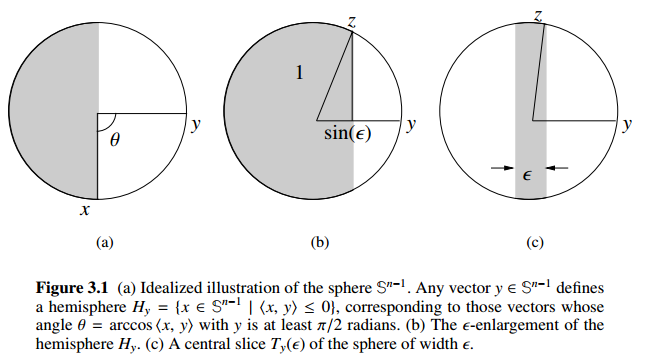
\includegraphics[scale = 0.5]{spherical_cap_blowup.png}}
\end{minipage}
\caption{\footnotesize{\textbf{spherical cap and $t$-blowup.   \citep{wainwright2019high}}}}
\label{fig: spherical_cap_blowup}
\end{figure}


\item \begin{definition} (\textbf{\emph{Spherical Cap and its $t$-Blowup}}) \\
Let $\bS^{n - 1} :=  \set{x \in \bR^n: \norm{x}{} = 1}$ be the \emph{$(n-1)$-dimensional \textbf{unit sphere}}. The \emph{\textbf{intersection}} of a \emph{\textbf{half-space}} and $\bS^{n-1}$ is called a \emph{\textbf{spherical cap}}. In particular, for some $y \in \bR^n$, denote the associated spherical cap as
\begin{align*}
H_y := \set{x \in \bS^{n-1}: \inn{x}{y} \le 0}
\end{align*} With some simple geometry, it can be shown that its  \emph{$t$-blowup}  corresponds to the set
\begin{align*}
H_y^{t} := \set{x \in \bS^{n-1}: \inn{x}{y} < \sin(t)}
\end{align*}
\end{definition}

\item \begin{theorem} (\textbf{Isoperimetry Theorem on Unit Sphere}) \citep{boucheron2013concentration, vershynin2018high, wainwright2019high}\\
Let $A$ be a subset of the sphere $\bS^{n-1}$, and let $\sigma$ denote the \textbf{normalized area} on that sphere. Let $t > 0$. Then,
among all sets $A \subset \bS^{n-1}$ with given area $\sigma(A)$, the \underline{\textbf{spherical caps}} \textbf{minimize}
\textbf{the area of the neighborhood} $\sigma(A_t)$, where
\begin{align*}
A_t := \set{x \in \bS^{n-1}: \exists y \in A \text{ such that } \norm{x - y}{} < t}
\end{align*}
\end{theorem}

\item \begin{remark}
Define a \emph{metric} $\rho$ on sphere $\bS^{n-1}$ as 
\begin{align*}
\rho(x, y) := \arccos(\inn{x}{y})
\end{align*}
Thus $(\bS^{n-1}, \rho)$ is a \emph{\textbf{metric space}}.  Let $\bP$ be uniform distribution on $\bS^{n-1}$ so that $((\bS^{n-1}, \rho), \bP)$ is a probability space. 
\end{remark}



\item \begin{proposition} (\textbf{Isoperimetric Inequalities for Uniform Distribution over Sphere})  \citep{boucheron2013concentration, vershynin2018high, wainwright2019high}\\
Let $\bS^{n - 1} :=  \set{x \in \bR^n: \norm{x}{} = 1}$ be the $(n-1)$-dimensional \textbf{unit sphere}.  For any $t\in [0, 1]$, 
\begin{align}
\alpha_{\bS^{n-1}}(t) &\le c \exp\paren{-\frac{n t^2}{2}} \label{ineqn: isoperimetric_inequality_uniform_unit_sphere}
\end{align} for some constant $c$.
\end{proposition}
\begin{proof}
Consider spherical cap 
\begin{align*}
C(y, 0) := \set{x \in \bS^{n-1}: \inn{x}{y} \ge 0}
\end{align*} and its  \emph{$t$-blowup}
\begin{align*}
C(y, t) :=  \set{x \in \bS^{n-1}: \inn{x}{y} \ge t}.
\end{align*} According to \emph{the isoperimetry theorem on unit sphere}, the concentration function for uniform distribution over $\bS^{n-1}$
\begin{align*}
\alpha_{\bS^{n-1}}(t) &= \bP(C(y, t)).
\end{align*} 

\begin{figure}
\begin{minipage}[t]{0.5\linewidth}
  \centering
  \centerline{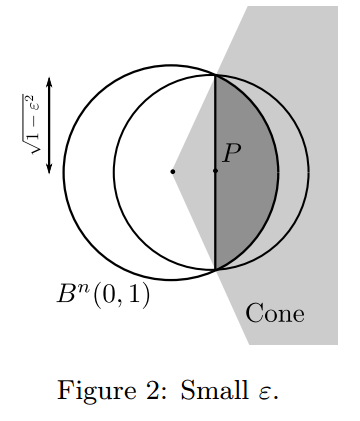
\includegraphics[scale = 0.4]{spherical_cap_proof.png}}
\end{minipage}
\begin{minipage}[t]{0.5\linewidth}
  \centering
  \centerline{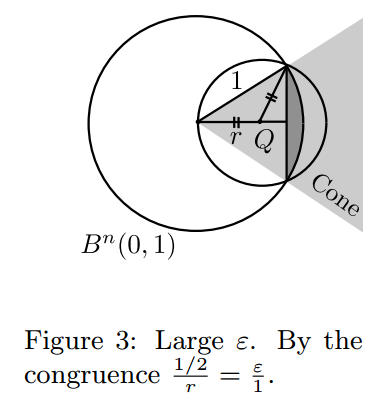
\includegraphics[scale = 0.4]{spherical_cap_proof_2.png}}
\end{minipage}
\caption{\footnotesize{\textbf{proof for upper bound of area of spherical cap (left) for small $t$ (right) for large $t$}}}
\label{fig: spherical_cap_blowup}
\end{figure}


Note that $\bP\paren{C(y, 0)} \le 1/2$.  In order to bound the concentration function from above, consider for small $t \in [0, 1/\sqrt{2}]$,
\begin{align*}
\alpha_{\bS^{n-1}}(t) = \bP\paren{C(y, t)} &= \frac{\text{Vol}(B^n(0, 1)\cap \text{Cone})}{\text{Vol}(B^{n}(0,1))} \\
&\le \frac{\text{Vol}(B^n(P,  \sqrt{1 - t^2}))}{\text{Vol}(B^{n}(0,1))}\\
&= (\sqrt{1 - t^2})^{n} \\
&\le \exp\paren{-  \frac{nt^2}{2}}
\end{align*}

For $t \in [1/\sqrt{2}, 1)$, it is enough to consider a different auxiliary ball which includes the set $\text{Cone} \cap B^n(0, 1)$. We obtain
\begin{align*}
\alpha_{\bS^{n-1}}(t) = \bP\paren{C(y, t)} & \le \frac{\text{Vol}(B^n(Q,  r))}{\text{Vol}(B^{n}(0,1))}\\
&= r^n = \paren{\frac{1}{2t}}^n\\
&\le \exp\paren{-\frac{n t^2}{2}}
\end{align*} where the last inequality is from $e^{x^2/2} \le 2x$ for $x \in [1/\sqrt{2}, 1]$. Due to convexity, this is only to be checked at the boundary of our interval
$[1/\sqrt{2}, 1]$,  \qed
%we see that $\sin(t) \ge t/2$ for $t \in (0, \pi/2]$. Then the $t$-blowup $H_y^{t}$ must contain set
%\begin{align*}
%\widetilde{H}_y^{t} := \set{x \in \bS^{n-1}: \inn{x}{y} < \frac{t}{2}},
%\end{align*} hence $\bP(\widetilde{H}_y^{t}) \le \bP(H_y^{t} )$. By geometric calculation, for all $t\in (0, \sqrt{2})$, we have 
%\begin{align*}
%\bP(\widetilde{H}_y^{t}) &\ge 1- \brac{1 - \paren{\frac{t}{2}}^2}^{n/2} \ge 1 - \exp\paren{-\frac{n\,t^2}{8}}
%\end{align*} where the last inequality is due to $(1 - x) \le e^{-x}$. Thus
%\begin{align*}
%\alpha_{\bS^{n-1}}(t) &= 1 - \bP(H_y^{t}) \le \exp\paren{-\frac{n\,t^2}{8}}.
%\end{align*} A similar but more careful approach to bounding $\bP(H_y)$ can be used to establish the sharper upper bound
%\begin{align*}
%\alpha_{\bS^{n-1}}(t) &\le  \sqrt{\frac{\pi}{2}}\exp\paren{-\frac{n t^2}{2}}. \qed
%\end{align*}
\end{proof}

\item By Levy's inequality, we have the following proposition
\begin{proposition} (\textbf{Lipschitz Function on $\bS^{n-1}$}) \citep{wainwright2019high}\\
For any $1$-Lipschitz function $f$ defined on the sphere $\bS^{n-1}$, we have the two-sided bound
\begin{align}
\bP\set{\abs{f(Z) - \text{Med}(f(Z))} \ge t} &\le \sqrt{2\pi}\exp\paren{-\frac{n t^2}{2}} \label{ineqn: lipschitz_unit_sphere_median}
\end{align} Moreover, replacing median by the mean, we have 
\begin{align}
\bP\set{\abs{f(Z) - \E{}{f(Z)} } \ge t} &\le 2\sqrt{2\pi}\exp\paren{-\frac{n t^2}{8}} \label{ineqn: lipschitz_unit_sphere_mean}
\end{align}
\end{proposition}

\item \begin{exercise} \textbf{(The Blow-Up Phenomenon)}\\
Let $A$ be a subset of the sphere $\sqrt{n} \bS^{n-1}$ such that
\begin{align*}
\bP\paren{A} > 2 \exp\paren{-c s^2} \text{ for some }s > 0;
\end{align*}
\begin{enumerate}
\item Prove that $\bP(A_s) > 1/2$.
\item Deduce from this that for any $t \ge s$,
\begin{align*}
\bP\paren{A_{2t}} > 1 - 2 \exp\paren{-c t^2}.
\end{align*} Here $c > 0$ is the absolute constant in upper bound of concentration function.
\end{enumerate}
\end{exercise}

\item \begin{remark} (\textbf{\emph{Zero-One Law for Independent Variables}}) \citep{vershynin2018high}\\
\emph{\textbf{The blow-up phenomenon}} we just saw may be quite \emph{counter-intuitive} at first sight. How can an exponentially small set $A$ undergo such a dramatic transition to an exponentially large set $A_{2t}$ under such a small perturbation $2t$ ? (Remember that $t$ can be much smaller than the radius $\sqrt{n}$ of the sphere.) 

However perplexing this may seem, this is \emph{a typical phenomenon in \textbf{high dimensions}}. It is \emph{reminiscent} of \textbf{\emph{zero-one laws}} in
\emph{probability theory}, which basically state that \emph{events that are determined by many random variables} tend to have \emph{probabilities either zero or one}.
\end{remark}
\end{itemize}
\subsection{Gaussian Isoperimetric Inequalities and  Concentration of Gaussian Measure}
\subsection{Edge Isoperimetric Inequality on the Binary Hypercube}
\subsection{Vertex Isoperimetric Inequality on the Binary Hypercube}
\subsection{Convex Distance Inequality}


%\section{The Classic Isoperimetry Inequalities}
%\subsection{Concentration of Lipschitz Function for the Sphere}






\newpage
\bibliographystyle{plainnat}
\bibliography{reference.bib}
\end{document}